\documentclass[titlepage]{jsarticle}
\usepackage[dvipdfmx]{graphicx}
\usepackage{h31ec-exp}
\usepackage{listings}
\lstset{
    basicstyle={\ttfamily},
    identifierstyle={\small},
    commentstyle={\smallitshape},
    keywordstyle={\small\bfseries},
    ndkeywordstyle={\small},
    stringstyle={\small\ttfamily},
    frame={tb},
    breaklines=true,
    columns=[l]{fullflexible},
    numbers=left,
    xrightmargin=0zw,
    xleftmargin=3zw,
    numberstyle={\scriptsize},
    stepnumber=1,
    numbersep=1zw,
    lineskip=-0.5ex,
    keepspaces=true,
    language=c
}
\renewcommand{\lstlistingname}{リスト}
\makeatletter
\newcommand{\figcaption}[1]{\def\@captype{figure}\caption{#1}}
\newcommand{\tblcaption}[1]{\def\@captype{table}\caption{#1}}
\makeatother

\title{電子回路設計・製作}
\grade{4年32番}
\author{平田 蓮}
\team{}
\date{2020年10月8日}
\expdate{2020年7月9日, 7月16日, 7月30日, 8月6日, 9月3日, 9月10日, 9月17日}
\coauthor{}

\begin{document}
\maketitle
\section{作品名}
    リアルタイム電卓

\section{構造}
    図\ref{fig:circuit}に作品図を示す.

    \begin{figure}[h]
        \centering
        \includegraphics[width=12cm]{img/circuit.png}
        \caption{作品図}
        \label{fig:circuit}
    \end{figure}

    回路はArduino, キーパッド, ブレッドボード, 16$\times$2液晶ディスプレイ, 180$\Omega$抵抗からなる.

\section{動作原理}
    回路の動作として, まず初めにキーパッドに入力があると, キーに対応した文字が液晶ディスプレイの上段に出力される.

    各キーと文字の対応は表\ref{tab:keys}の通りである.

    \begin{table}[h]
        \centering
        \caption{キーと文字の対応}
        \label{tab:keys}
        \begin{tabular}{c|c}
            キー & 文字 \\ \hline
            1 〜 9 & 1 〜 9 \\
            A & + \\
            B & - \\
            C & ( \\
            D & ) \\
            ** & * \\
        \end{tabular}
    \end{table}

    \#キーについては, 文字が出力されるわけではなく, 液晶ディスプレイの出力が1文字削除される.

    入力が行われるたびに, 液晶ディスプレイの上段の数式が評価される.
    もし数式が成り立っている場合, その数式の計算結果が液晶ディスプレイの下段に出力される.

\section{ハードウェア}
    図\ref{fig:circuit2}に回路図を示す.

    \begin{figure}[h]
        \centering
        \includegraphics[width=12cm]{img/circuit2.png}
        \caption{回路図}
        \label{fig:circuit2}
    \end{figure}

    回路は文献\cite{circuit}を参考にした.

    液晶ディスプレイには180$\Omega$の抵抗を接続してある.
    これは, 電源電圧を5V, LEDの順方向電圧を1.7V, LEDの順方向電流を20mAとしたときに次のように計算できる.

    \begin{equation}
        \frac{5 - 1.7 \ \mathrm{V}}{20 \times 10^3 \ \mathrm{A}} = 165 \ \Omega
    \end{equation}

    理論上は165$\Omega$の抵抗を使えばいいことになるが, 今回は最も近い値を持つE24系列の抵抗として180$\Omega$
    のものを使った.

\section{ソフトウェア}
    図\ref{fig:flowchart}に動作のフローチャートを示す.

    \begin{figure}[h]
        \centering
        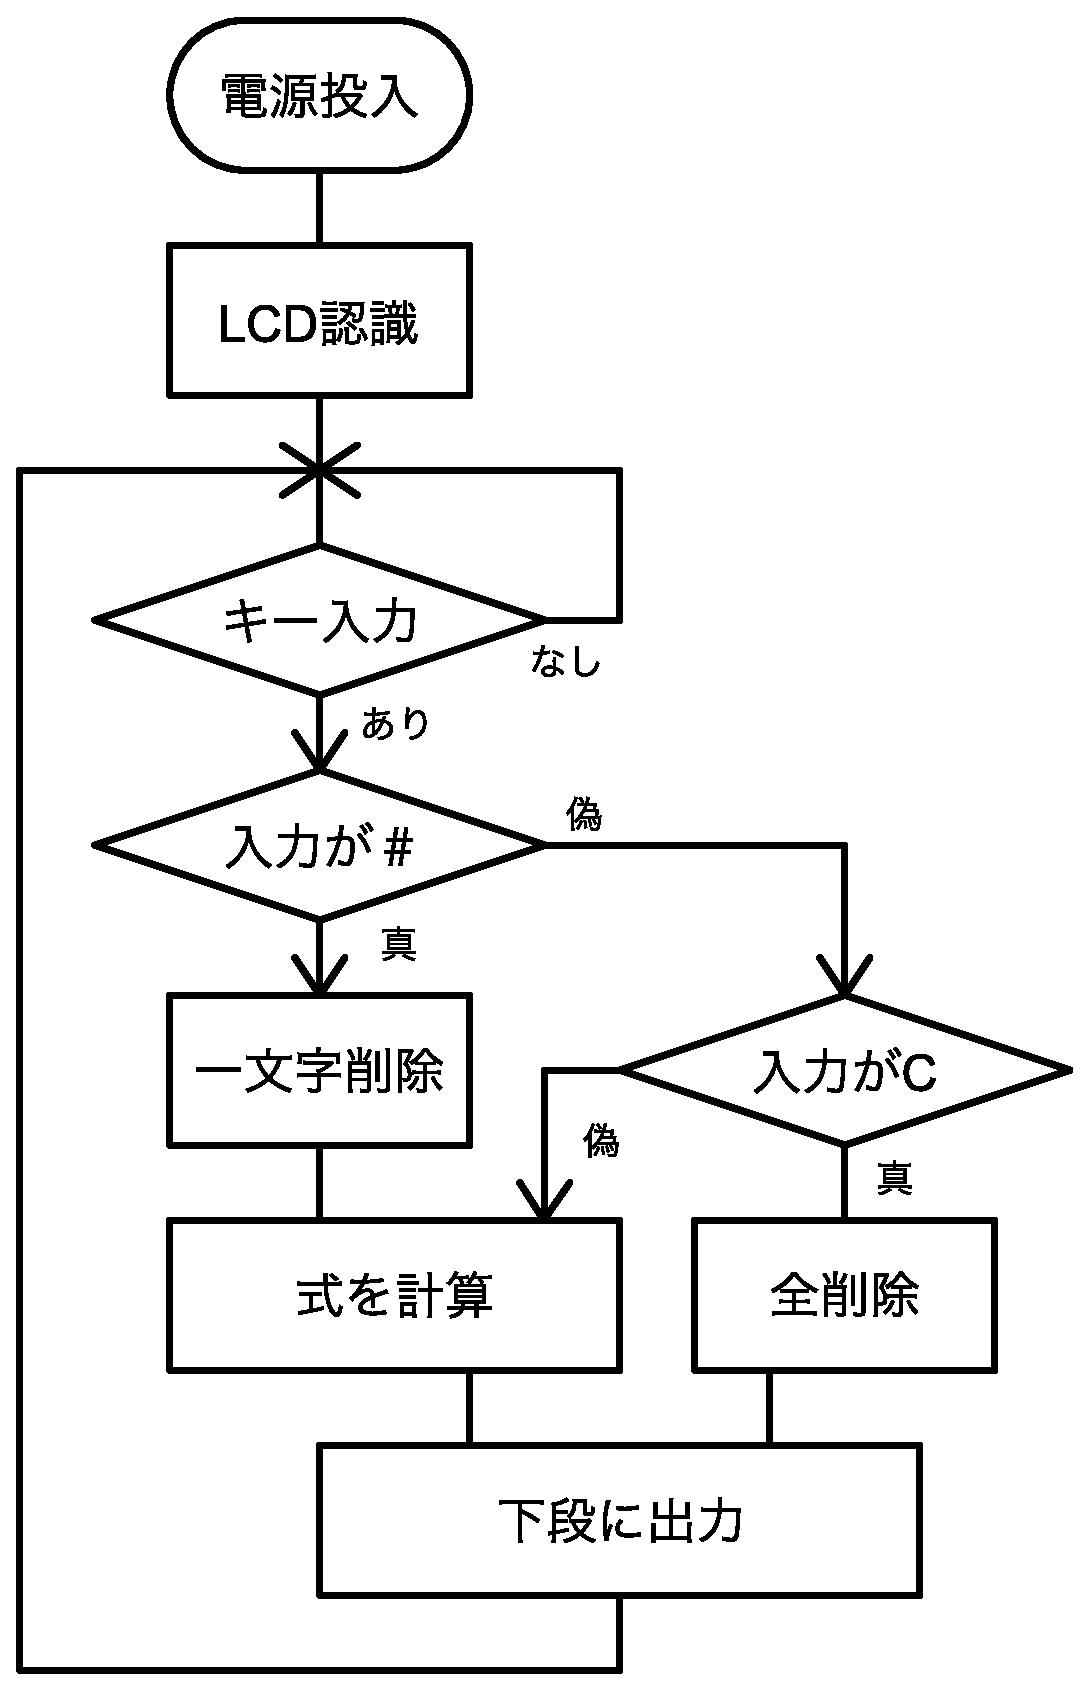
\includegraphics[width=8cm]{img/flowchart.eps}
        \caption{フローチャート}
        \label{fig:flowchart}
    \end{figure}

    このフローチャートを元に作成したソースコードをリスト\ref{src:code}に示す.

    \begin{lstlisting}[caption=ソースコード, label=src:code]
#include <Keypad.h>
#include <LiquidCrystal.h>

LiquidCrystal lcd(5, 4, 3, 2, A4, A5);

const byte ROWS = 4;
const byte COLS = 4;
char keys[ROWS][COLS] = {
    {'1', '2', '3', '+'},
    {'4', '5', '6', '-'},
    {'7', '8', '9', '('},
    {'*', '0', '<', ')'}
};
byte row_pins[ROWS] = {A0, A1, 11, 10};
byte col_pins[COLS] = {9, 8, 7, 6};
Keypad keypad = Keypad(
    makeKeymap(keys),
    row_pins,
    col_pins,
    ROWS,
    COLS
);

int lcd_frame = 0;
char content[20] = {};

void setup(){
    lcd.begin(16, 2);
}


int calc(char* content) {
    int a = 0, b, j = 0;
    int sanitized[20] = {};
    
    for (int i = 0; i < lcd_frame; i++) {
        if (content[i] >= '0' && content[i] <= '9') {
            a *= 10;
            a += content[i] - '0';
        } else {
            if (a) {
                sanitized[j] = a;
                j++;
                a = 0; 
            }
            
            if (content[i] == '+') {
                sanitized[j] = -1;
            } else if (content[i] == '-') {
                sanitized[j] = -2;
            } else if (content[i] == '*') {
                sanitized[j] = -3;
            } else if (content[i] == '(') {
                sanitized[j] = -4;
            } else {
                sanitized[j] = -5;
            }
            j++;
        }
    }
    
    if (a) {
        sanitized[j] = a;
        j++;
    }
    
    int s[20] = {}, q[20] = {}, s_ptr = 0, q_ptr = 0;
    for (int i = 0; i < j; i++) {
        if (sanitized[i] >= 0) {
            q[q_ptr] = sanitized[i];
            q_ptr++;
        } else if (sanitized[i] > -4) {
            s_ptr--;
            while (
                s_ptr >= 0 &&
                s[s_ptr] < sanitized[i] &&
                s[s_ptr] > -4
            ) {
                q[q_ptr] = s[s_ptr];
                q_ptr++;
                
                s[s_ptr] = 0;
                s_ptr--;
            }
            s[++s_ptr] = sanitized[i];
            s_ptr++;
        } else if (sanitized[i] == -4) {
            s[s_ptr] = sanitized[i];
            s_ptr++;
        } else {
            s_ptr--;
            while (
                s_ptr >= 0 &&
                s[s_ptr] != -4
            ) {
                q[q_ptr] = s[s_ptr];
                q_ptr++;
                
                s[s_ptr] = 0;
                s_ptr--;
            }
            
            if (s[s_ptr] == -4) {
                s[s_ptr] = 0;
                s_ptr--;
            }
        }
    }
    
    while (s_ptr >= 0) {
        if (s[s_ptr] != 0) {
            q[q_ptr] = s[s_ptr];
            q_ptr++; 
        }
        
        s[s_ptr] = 0;
        s_ptr--;
    }
    
    s_ptr = 0;
    for (int i = 0; i < q_ptr; i++) {
        if (q[i] >= 0) {
            s[s_ptr] = q[i];
            s_ptr++;
        } else {
            s_ptr--;
            b = s[s_ptr];
            s[s_ptr] = 0;

            s_ptr--;
            a = s[s_ptr];
            s[s_ptr] = 0;
            
            if (q[i] == -1) {
                s[s_ptr] = a + b;
            } else if (q[i] == -2) {
                s[s_ptr] = a - b;
            } else {
                s[s_ptr] = a * b;
            }
            s_ptr++;
        }
    }
    return s[0];
}

void loop(){
    const char key = keypad.getKey();
    
    if (key == '<') {
    lcd.clear();
        lcd.setCursor(0, 0);
        lcd_frame--;
        content[lcd_frame] = '\0';

        for (int i = 0; i < lcd_frame; i++) {
            lcd.print(content[i]);
        }
    } else if (key) {
        if (lcd_frame < 16) {
            lcd.setCursor(lcd_frame, 0);
            content[lcd_frame++] = key;
            lcd.print(key);
        }
    }

    lcd.setCursor(0, 1);
    lcd.print(calc(content));
}\end{lstlisting}

    \verb|calc()|は与えられた文字列を数式としてみたときにその結果を計算する関数である.
    式を処理する際に操車場アルゴリズム\cite{shunt}というものを利用した.

    実際のアルゴリズムではキューとスタックを使用するが,
    Arduino内部のライブラリでキューやスタックは実装されていないようなので,
    通常の配列とポインタで代用した.

    操車場アルゴリズムを適用した文字列は後置記法となる.
    110行目から143行目では再びスタックを使用して後置記法となった式の計算をしている.

\section{結果・今後の課題}
    結果として, 満足する動作をさせることができたと思う.
    細かい動作にバグなどがあるかもしれないので, 今後をそれらを調べていきたい.

    また, 今回は除算は表示桁数が長くなると予想したため実装しなかったが,
    実装してみるのも面白いと思う.
    その場合は0での除算を防がないといけないのですこし手間がかかるかもしれない.

\section{感想}
    今回は電子回路設計ということであったが,
    どちらかというと回路のハードウェアというよりArduino内部のコードに時間をかけた.
    今年は実際の回路を組むわけではなくオンライン上で作業をしたということもあり,
    使える部品が豊富にあった.
    もし次にTinkercad Circuitsを使うようなことがあれば今度はハードウェアに寄せた回路を作ってみたい.

\begin{thebibliography}{99}
    \bibitem{circuit} Invincible Academy, Keypad Interfacing in Tinkercad https://www.youtube.com/watch?v=pyBRSLCXmoQ
    \bibitem{shunt} @HMMNRST, 操車場アルゴリズムで四則計算の数式をパース \\ 
        https://qiita.com/HMMNRST/items/e42a2062eb3bb6f46d37
\end{thebibliography}

\end{document}